\chapter{Results} % (fold)
\label{sg:cha:results}

% 1
% ========================================================
% = the analysis of synergies in the nonevoked condition =
% ========================================================		
\section{Synergies during natural movement} % (fold)
\label{sg:sec:nat_mov_syns}

% preprocessing, response patterns, rank1

For all monkeys together there is data from in total 116 sessions available. Sessions were excluded from further analysis when one of the following criteria was met: data from only less then 50 trials available, preferred directions unstable over sessions or the remaining-error of the rank 1 model was already less then 25 \%. For subject V all sessions were done in pronation hand-position. 
\todo{explain what unstable pd means (more than 4 channels more than 2 stds away from mean pd over sessions)}

% table of all available data 
\begin{table}[ht]
	\centering
	\begin{tabular}{r|c|c|c}
		\toprule
		                    & vega  & darma & chalva \\
		\toprule
		total               & 91    & 10    & 15\\
		\midrule
		less than 50 trials & 2     & 0     & 0\\
		\midrule
		unstable pds        & 8     & 0     & 1\\
		\midrule
		rank1               & 2     & 0     & 0\\
		\bottomrule
		remaining           & 79    & 10    & 14\\		
		\bottomrule
	\end{tabular}
	\caption{}
	\label{sg:tab:sorting_table}	
\end{table}

\todo{mean number of trials: 291.9138  (put this into text)}
After the computation of relative activation, the data was in form of a $\text{trials} \times \text{channels}$ matrix for each session and hand position. The whole subsequent analysis was always performed in parallel for separated hand positions and also for a $\text{supination trials} + \text{pronation trials} \times \text{channels}$ matrix, containing the data for both hand positions. First the MF-algorithms were applied to the matrices containing both hand-positions trying to reduce the dimensionality of the data to only one synergy (rank 1 model order). This was done in order to sort out sessions were EMG signals across channels are highly correlated. The PCAICA-algorithm led to generally smaller error values, but they were highly correlated with the remaining error values of the NMF-algorithm (r: 0.85, p << 0.001). NMF was, due to its biologically plausible assumptions, preferred in the further analysis and therefore also chosen for selection of sessions. The threshold of remaining error in order to qualify for further analysis was set to 25 \% as it seemed to be a reasonable tradeoff between amount of data and information contained in the data. The selection was done by using the pronation position as supination was not available for all sessions and the two conditions are also highly correlated (r: 0.77, p << 0.001).

% rank 1 figure
\begin{figure}[ht]
	\centering
		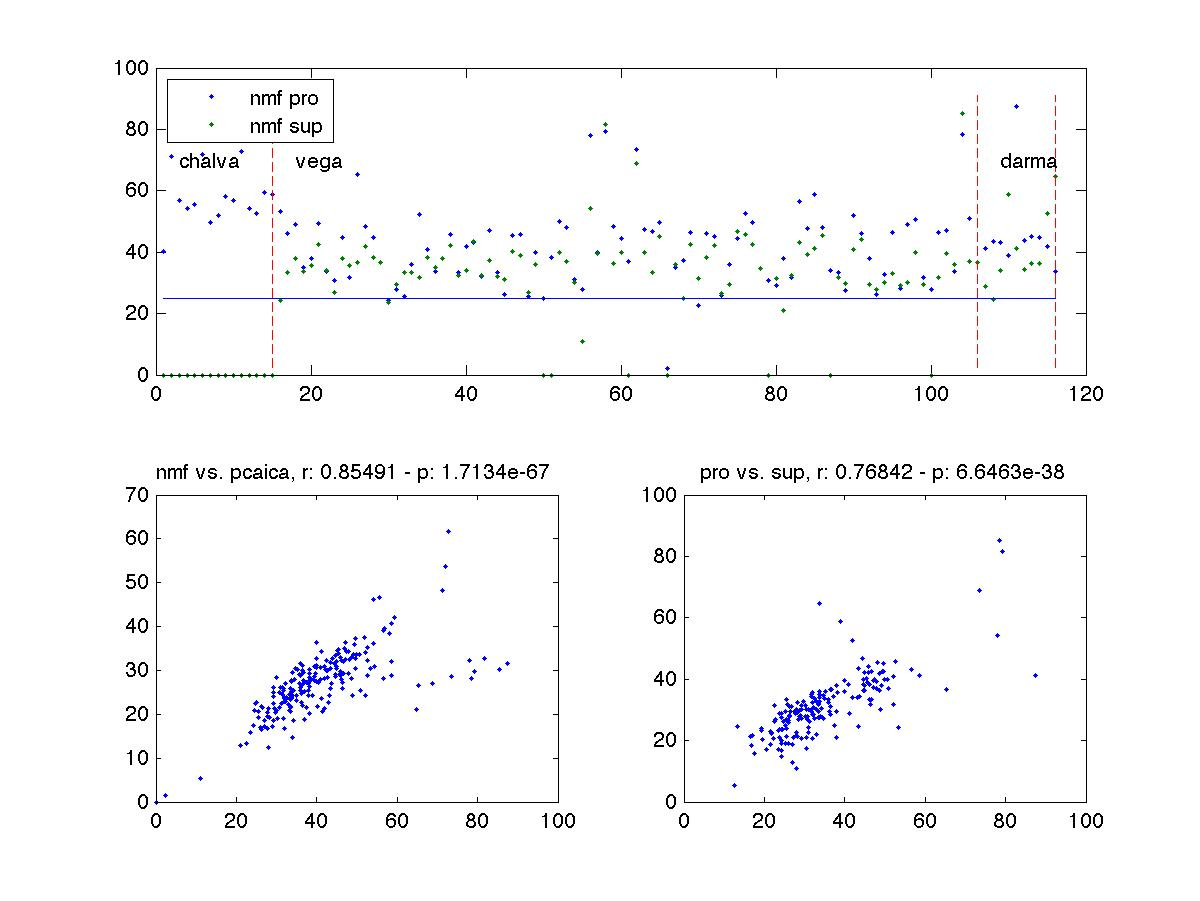
\includegraphics[width=0.7\textwidth]{images/rank1.jpg}
	\caption{
Error values for NMF in pronation and supination when data was reduced to a 1 dimensional model. Sessions with an NMF remaining error higher than 25 \% were chosen for further analysis.
	}
	\label{sg:fig:images_rank1}
\end{figure}


% synergy computation for separated sessions
The NMF remaining error plot suggests, that the data for each session can be reduced to 3 dimensions while still explaining 85 \% of the  variance~\rref{sg:fig:images_all_resid_non}. It also shows that this is due to the structure of the data as random data with same statistical properties leads to higher error values. Examination of PCAICA error values led to the same results but is not shown here because of the strong correlation between the two measurements in the rank 1 analyses~\rref{sg:fig:images_rank1}.
% all resid nonevoked figure
\begin{figure}[ht]
	\centering
		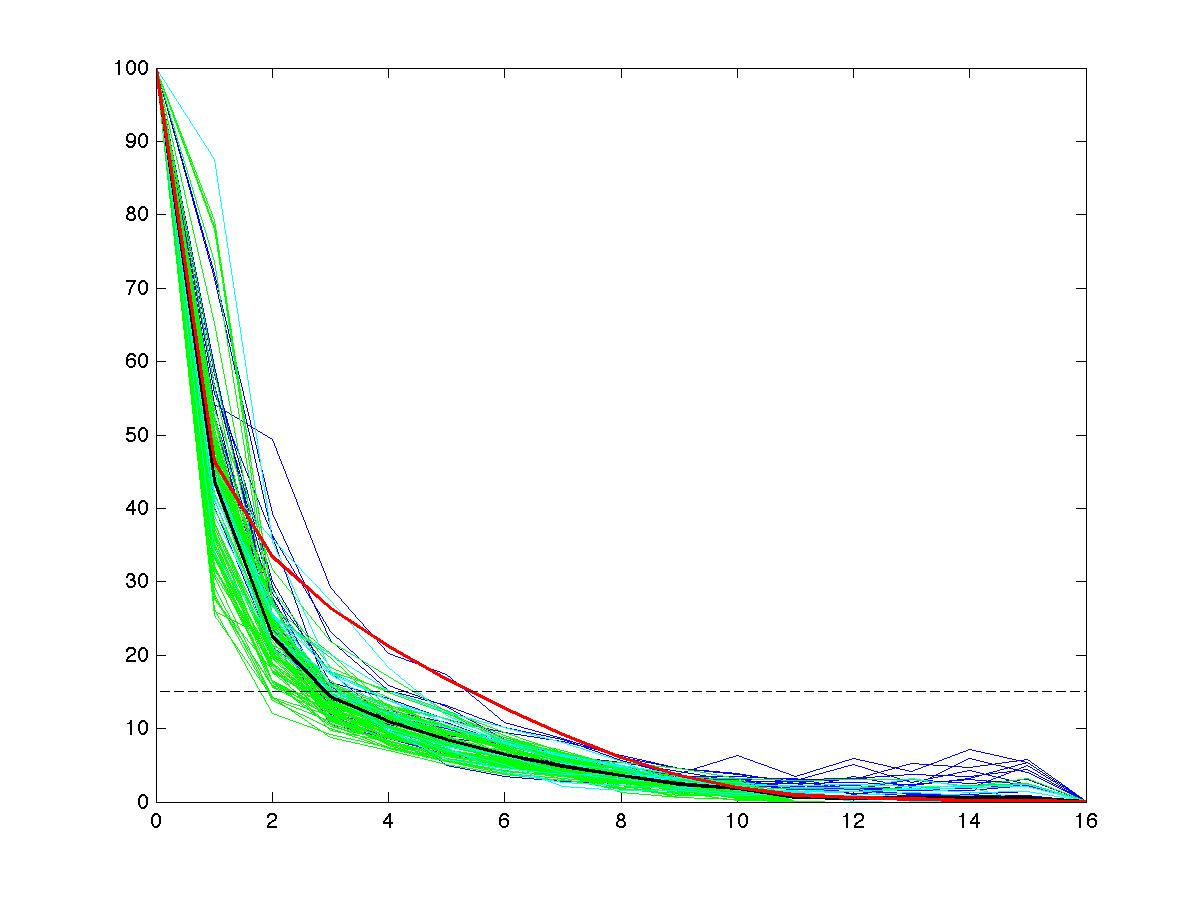
\includegraphics[width=0.9\textwidth]{images/resid_test.jpg}
	\caption
	{
	remaining error for data from pronation hand-position has 15 \% remaining error if reduced to a 3 dimensional model. Randomized data with same statistical properties (shuffled data) shows much higher error values.
	}
	\label{sg:fig:images_all_resid_non}
\end{figure}

To assess the stability of the synergies over sessions, all synergies extracted from single sessions were as in the method to compare NMF stability~\rref{sg:fig:images_nmf_expl_stab3} pooled in one data set and sorted according to a k-means clustering with 3 prototypes. The distribution of group size does not exhibit perfect categorization (STD 0) as in the stability analyses but still shows clear clustering and therefore stable muscle synergies over sessions. The prototypes of the k-means clustering are the average synergies steadily found over all sessions. This analysis was done for the pronation hand-position as this was available for all monkeys


% nmf stability over sessions (cluster std)
\begin{figure}[h]
    \centering
    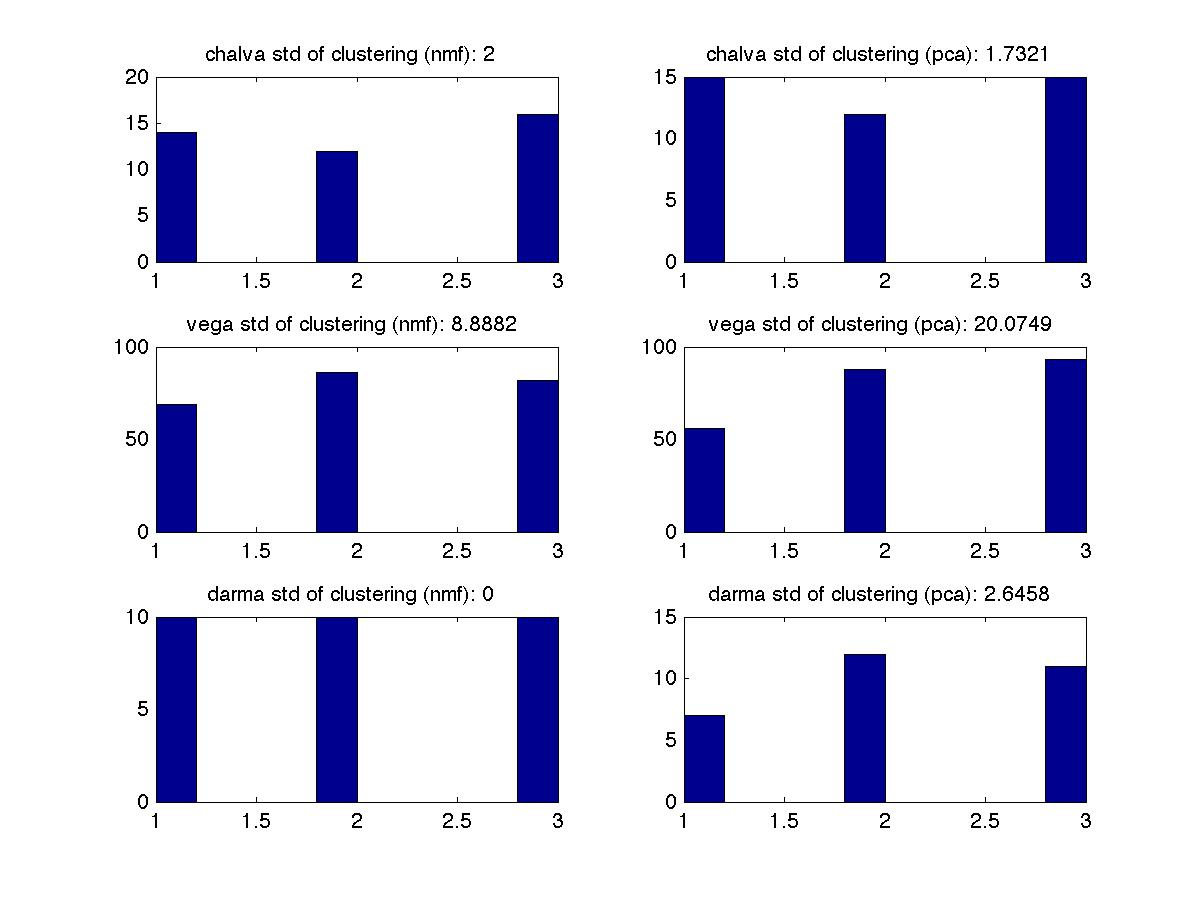
\includegraphics[width=0.8\textwidth]{images/syn_consist_sessions_std.jpg}
    \caption{Distribution and std of the group sizes when clustering the synergies obtained from different sessions}
    \label{sg:fig:images_syn_consist_sessions_std}
\end{figure}


% consist over sessions and method explanation plot (chalva)
\begin{figure}[h]
    \centering
    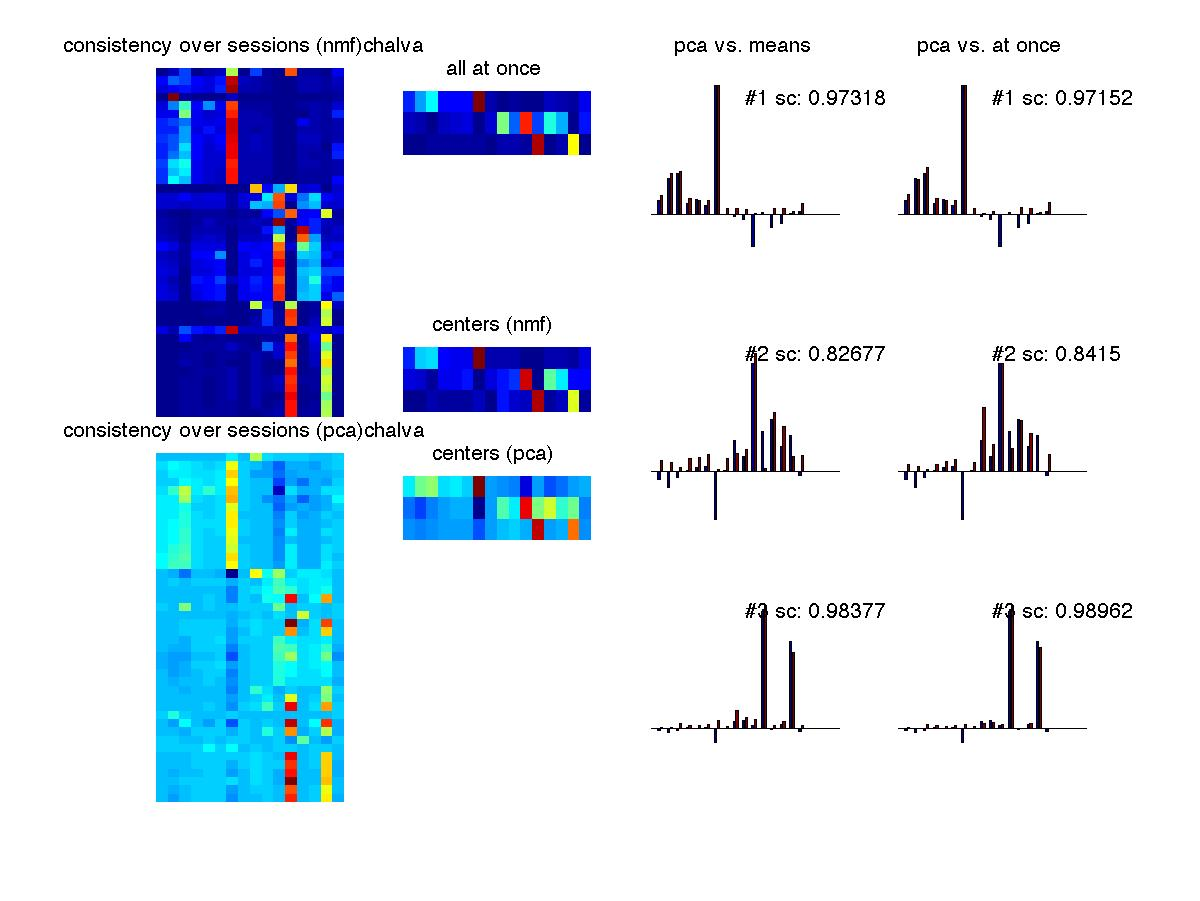
\includegraphics[width=0.8\textwidth]{images/syn_consist_sessions_chalva.jpg}
    \caption{
    all data in this plot is from pronation hand-position 
    \textbf{a)} The stability of extracted synergies over sessions was assessed similar to the stability measure of the MF-algorithm~\rref{sg:fig:images_nmf_expl_stab3}. All results were pooled and clustered by a k-means algorithm with the number of prototypes corresponding to the number of synergies. Similarity within the three blocks demonstrates stability over sessions. The strength of activation is coded by color. Note that color-coding is distinct for NMF- and PCAICA extracted synergies as NMF gives only positive results.synergies sorted according to cluster membership for both methods 
    \textbf{b)} comparison of cluster means and when computed the synergies on all data at once 
    \textbf{c)} pca vs. nmf means 
    \textbf{d)} pca vs. nmf all at once 
    }
    \label{sg:fig:images_syn_consist_sessions_chalva}
\end{figure}
\todo{nicer plot, maybe even one for all monkeys together. look at corresponding plot in ba thesis}
\todo{give numbers for the two other monkeys in a table}


\todo{show plot of posture similarity}



To sum up, it was possible to extract 3 muscle synergies from data, which was collected from many sessions of natural movement.
The extracted synergies proved to be similar over different hand postures and were reliably found from different algorithms of
matrix factorization. This is consistent with the findings of other publications that were mentioned in the introduction.



%output off all remaining pictures of this section
\clearpage

% section nat_mov_syns (end)


% 1
% ===============================================================
% = analysis if synergies from respones to cortical stimulation =
% ===============================================================
\section{Synergies in the evoked responses} % (fold)
\label{sg:sec:evoked_syns}

Within the 62 \todo{adapt the numbers in the whole paragraph to the 3 monkeys, maybe a table} recording-sessions for which EMG data was available, 211 sub-sessions with cortical microstimulation in different sites took place. For each sub-session average response windows around stimulation time were computed and after visual inspection the sub-sessions containing artifacts in the window were sorted out so that 160 remained. As described before, arm-related areas were mapped by trains of stimulating pulses and the observation of visible responses (jerking of muscles) to this stimulation. This method could serve only for very coarse mapping as muscle activation is not necessarily visible. Therefore muscle field sizes of responses were calculated which give a more objective method for detection of arm-related locations in the cortex. Sub-sessions with a muscle field size of 0 (no significant response) were also sorted out which left 134 sub-sessions for synergy analysis, 72 of them recorded while the hand was held in pronation and 61 while hand was held in supination posture.
A distribution of muscle field size can be seen in figure~\rref{sg:fig:images_resp_fields}  and a plot of the muscle field size in relation to stimulation site in section \emph{b}. In this plot it becomes visible that the preliminary coarse mapping is not perfectly reliable as even sites that showed facial or no response can have significant and large muscle fields. However muscle fields are generally larger in stimulation sites mapped to finger or wrist movements. 
\todo{add a plot like this} 
% CAPTION The relation between muscle field size and the site of stimulation. Note that even sites that showed observable responses in facial areas during the coarse mapping might exhibit significant muscle fields.
In each location, stimulation was applied with different stimulation amplitudes (from minimum 50 up to 250 $\mu A$) but not in all locations with all amplitudes. For each location the stimulation amplitude closest to $150 \mu A$ was chosen as most data was available around this strength~\rref{sg:fig:stimamp_dist} \emph{c}.

\begin{figure}[ht]
    \centering
        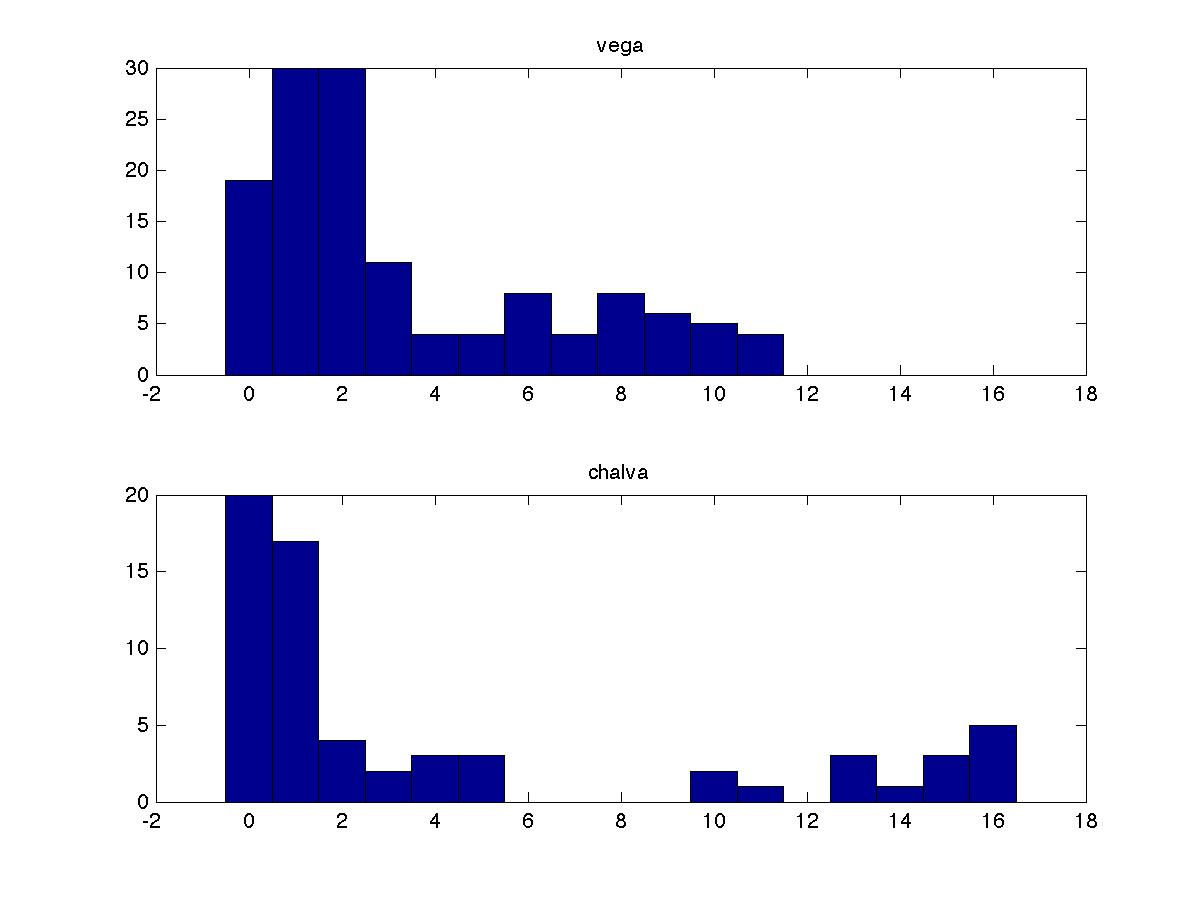
\includegraphics[width=0.8\textwidth]{images/resp_fields.jpg}
    \caption{The distribution of muscle field size.}
    \label{sg:fig:images_resp_fields}
\end{figure}

% figure of muscle field distribution, locations and stim amp distribution
\begin{figure}[ht]
	\centering
		\includegraphics[width=0.9\textwidth]{images/stimamp_dist.jpg}
	\caption{
		For each location the stimulation amplitude closest to $150 \mu A$ was chosen. The distribution shows the actually chosen stimulation amplitudes as $150 \mu A$ was not available for all locations.}
	\label{sg:fig:stimamp_dist}
\end{figure}

Again prior to the extraction of synergies, a remaining error test was done in order to find out to which dimension the data might be reduced while still explaining most of the variance. The remaining error plot was computed with both the PCA- and the NMF-algorithm. Both curves show an \emph{elbow} and suggest to reduce the dimensionality of the data to 2 or 3 motor-primitives. To facilitate comparison with the synergies extracted from natural movement a
reduction to 3 synergies was chosen. When the algorithms were applied to random data with same statistical properties
the error values remain higher, showing that the data contains structure. PCAICA again has generally smaller remaining
error values but also here the NMF was preferred due to its assumptions better suiting the data. 
\begin{figure}[ht]
	\centering
		\includegraphics[width=0.8\textwidth]{images/resid.pdf}
	\caption{Remaining error plot on the data from evoked muscle responses for model order selection. }
	\label{sg:fig:images_resid}
\end{figure}


Both algorithms extract similar synergies, shown by the correlation of the results~\rref{sg:fig:images_evo_pca_nmf_comp}. It is of note that
the matching score between synergies are not of the same value for all of the synergies. Apparently for pronation
and combined data always two synergies extracted by different algorithms fit better than a third one.
This might have different causes as it might result from noise or insufficient amount of data or from
selection of model with wrong order. The criteria for model order selection was not that clear in the remaining
error plot of the evoked responses. The unstable synergy might be the one with the smallest amount of explaining variance
and therefore might not be as stable as the others, yet this is not a satisfying explanation why this effect is not observed
in the supination posture.
% figure: comparison between pca and nmf synergies
\begin{figure}[ht]
	\centering
		\includegraphics[width=0.9\textwidth]{images/evo_pca_nmf_comp.pdf}
	\caption{Comparison of synergies extracted by different algorithms. The data from which synergies are computed
	was recorded during cortical stimulation when the hand of the monkey was hold in either pronation or supination posture.
	In the data from pronation and the combined pronation and supination data there is one synergy with weak similarity
	between PCAICA and NMF.}
	\label{sg:fig:images_evo_pca_nmf_comp}
\end{figure}


The comparison of synergies from stimulation where the hand of the monkey was held in different postures shows
an interesting result. It was expected that the muscle synergies would be independent of hand-posture. 
However both NMF and PCAICA extract synergies in different postures that do not all completely fit. 
The synergies in the comparison plot between postures~\rref{sg:fig:images_evo_between_pos_synrelation_pca} are extracted
by the PCAICA-algorithm as the synergies that also contain negative values show more reliable matching scores~\sref{sg:sec:syn_comp}.
In both algorithms it is one synergy that exhibits differences between different postures, the other two synergies
are always stable. This is probably caused by the same reasons that account for the low matching score of the 
not fitting synergy in the PCAICA - NMF comparison. However it might also be due to integration of sensory
information about hand posture in the corticospinal pathway and should be subject to further analysis in future studies. 
% figure comparison between postures
\begin{figure}[ht]
	\centering
		\includegraphics[width=0.6\textwidth]{images/evo_between_pos_synrelation_pca.pdf}
	\caption{Comparison between synergies extracted by PCAICA-algorithm from data recorded during cortical stimulation
	where the hand of the monkey was held in either pronation or supination posture.}
	\label{sg:fig:images_evo_between_pos_synrelation_pca}
\end{figure}


To see whether the muscle activation patterns follow a topographical organization in the motor cortex,
the distance between stimulation sites was correlated with the similarity of activation patterns.
The measure for muscle activation similarity was simply the distance between two activation patterns
in the space of muscle activations (L2-norm). The distance between sites was restricted to $5 mm$ as similarity
between more distant sites was not expected. No topographical organization could be found by this method.



% section evoked_syns (end)




% ============================================================
% = synergy relation, synergies in pd space, projection, etc =
% ============================================================
\section{Relation between evoked activation patterns and natural movement} % (fold)
\label{sg:sec:synergy_relations}

The preferred directions that were computed for each muscle in each recording session showed to
be stable over recording days. In channel 8 only a few computed PDs were significant because
this channel was corrupted by noise in many sessions. It was therefore not used in any analysis that
used preferred directions. There is a significant and also visually obvious difference of preferred directions
depending on the posture of the hand~\rref{sg:fig:images_pd_consist_feather}. 
As the PDs showed to be stable over recording sessions, for each muscle the average over sessions was
computed and used for further analysis.
\begin{figure}[ht]
	\centering
		\includegraphics[width=0.8\textwidth]{images/pd_consist_feather.pdf}
	\caption{Preferred directions of muscles are distinct in relation to hand-posture, but show consistent
	orientation over sessions. Channel 8 was very noisy in general and did not allow to compute preferred directions.}
	\label{sg:fig:images_pd_consist_feather}
\end{figure}


It was thought that the circular standard deviation of muscle synergies in the 
space of preferred directions can be used to assess whether the result of matrix-factorization
algorithms is realistic with respect to natural movement. The idea was that meaningful muscle activation patterns 
should have a lower \emph{cstd} than random activation patters in order to initiate movement in certain directions. 
The \emph{cstd} was computed for all synergies of single sessions, the average synergies of all single sessions, the synergies
computed on the pooled muscle activation patterns of all sessions and also the synergies which
were extracted from the evoked responses. For none of these synergies a significantly smaller circular standard deviation 
than for random data was found. 
As the PDs proved to be significant and the synergies were stably extracted by different algorithms,
the reason for this result has to be found within the directedness measurement or in the this measurement
underlying assumptions that muscle activation patterns correspond to directed movement.
Within the current approach, a lot of averaging takes place during computation. First the PD for 
a muscle is computed by a vector summation, then this PD is averaged over all significant session
and finally this computed PD is assigned to a muscle in an activation pattern,
only scaled in length by the value of the activation. As a lot of information is lost within this process,
direct basis approaches or probabilistic methods might be more promising.
However, it could also be that the assumption that meaningful muscle activation patterns should correspond to
directed movement is completely wrong. There could be a meaningful muscle activation pattern
which has two modes of activation each pointing to a different point in space.
The purpose of this muscle co-activation into opposing directions could be to increase
joint stiffness. In this case the circular variance will be very high, but the synergy would be still meaningful. 
More promising measures for the meaningfulness of muscle activation patterns will be proposed in the outlook part
of this thesis.

In order to compare the evoked responses with the synergies found during natural movement evaluation of projections 
onto different subspaces was applied. The natural movement synergies computed on the pooled data from all sessions
were used for this method. The data from evoked responses was projected onto the orthonormalized subspace that is spanned
by the synergies and also on its orthogonal complement. The ratio of the vector sums of the data projected onto the two subspaces
was for the evoked responses significantly higher than for random or randomized data. Although it is not a quantitative measure
that gives a value for the relation between the two, the result suggests that there is a significant relation between the muscle 
response patterns, evoked by cortical stimulation and the synergies extracted from natural movement. 
\begin{figure}[ht]
	\centering
		\includegraphics[width=0.5\textwidth]{images/projection.pdf}
	\caption{Projection ratios of evoked responses, compared to 10000 runs of data with same statistical properties and shuffled 
	versions of itself}
	\label{sg:fig:images_projection}
\end{figure}




% section synergy_relations (end)


\bigskip

\begin{table}[hb]
 \centering
 \begin{tabular}{ r p{10cm}}
  \toprule
  	62  	& 	sessions in which EMG data was not corrupted and data for both hand-positions was available\\
  	28 		& 	sessions in which the remaining error of a rank 1 NMF model was larger than 25 \%\\
	\toprule
	211 	& sub-sessions in which cortical microstimulation took place \\
	160  	& not corrupted by visible artifacts\\
	134		& with a muscle response field larger than 0\\
	\midrule
	72 		& in pronation hand-position\\
	61 		& in supination hand-position\\
	\bottomrule
 \end{tabular}
 \caption{General session statistics}
 \label{tab:non_evo_sess_stat}
\end{table}



% section results (end)
